\section{Bilinear forms and linear mappings}

Let \((\mathrm{F}_{1},\mathrm{G}_{1}),(\mathrm{F}_{2},\mathrm{G}_{2})\) be two pairs of (real or complex) vector spaces in separating duality (TVS, II, §6, No.~1); assume each of these spaces to be equipped with the corresponding weak topology (loc. cit., No.~2); if A and B are any two of these spaces, as usual we denote by \(\mathcal{L}(\mathrm{A};\mathrm{B})\) the vector space of continuous linear mappings of A into B, and by \(\mathfrak{B}(\mathrm{A},\mathrm{B})\) the vector space of separately continuous bilinear forms on \(\mathrm{A}\times \mathrm{B}\) .

For every separately continuous bilinear form \(\Phi\) on \(\mathrm{F}_1\times \mathrm{F}_2\) , \(x_{1}\mapsto \Phi (x_{1},x_{2})\) is a continuous linear form on \(\mathrm{F}_1\) , therefore there exists one and only one element \(^r\Phi (x_2)\in \mathbf{G}_1\) such that

\[
\Phi (x _ {1}, x _ {2}) = \langle x _ {1}, ^ {r} \Phi (x _ {2}) \rangle\tag{1}
\]

for \(x_{1} \in F_{1}\) , \(x_{2} \in F_{2}\) (TVS, III, §5, No.~1, (1)). Moreover, this formula shows that the mapping \(x_{2} \mapsto {}^{r}\Phi(x_{2})\) is linear and continuous for the (weak) topologies of \(F_{2}\) and \(G_{1}\) . Conversely, for every continuous linear mapping u of \(F_{2}\) into \(G_{1}\) , \((x_{1}, x_{2}) \mapsto \Phi(x_{1}, x_{2}) = \langle x_{1}, u(x_{2}) \rangle\) is a separately continuous bilinear form on \(F_{1} \times F_{2}\) , and \(^{r}\Phi = u\) . One thus defines an isomorphism \(r : \Phi \mapsto {}^{r}\Phi\) of \(\mathfrak{B}(F_{1}, F_{2})\) onto \(\mathcal{L}(F_{2}; G_{1})\) , said to be canonical.

Similarly, the formula

\[
\Phi (x _ {1}, x _ {2}) = \langle^ {l} \Phi (x _ {1}), x _ {2} \rangle\tag{2}
\]

defines a canonical isomorphism \(l: \Phi \mapsto {}^{l} \Phi\) of \(\mathfrak{B}(F_{1}, F_{2})\) onto \(\mathcal{L}(F_{1}; G_{2})\) ; and one obviously has the commutative diagram

\pandocbounded{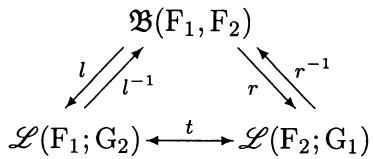
\includegraphics[keepaspectratio]{images/part003_fb3d81cd.jpg}}

where t is the isomorphism of transposition \(u \mapsto {}^{t}u\) . In view of the definition of the weak topologies on \(G_{1}\) and \(G_{2}\) , it is moreover immediate that when \(\mathfrak{B}(F_{1}, F_{2})\) , \(\mathcal{L}(F_{1}; G_{2})\) and \(\mathcal{L}(F_{2}; G_{1})\) are equipped with the topology of pointwise convergence, the isomorphisms in the preceding diagram are isomorphisms for the topological vector space structures.

Now let E, F be two Hausdorff locally convex spaces, \(E'\) , \(F'\) their respective duals; we denote by \(E_{\sigma}\) , \(F_{\sigma}\) the spaces E, F equipped with the weakened topologies \(\sigma(\mathrm{E}, \mathrm{E}')\) , \(\sigma(\mathrm{F}, \mathrm{F}')\) , and by \(E_{s}'\) , \(F_{s}'\) the spaces \(E'\) , \(F'\) equipped with the weak topologies \(\sigma(\mathrm{E}', \mathrm{E})\) , \(\sigma(\mathrm{F}', \mathrm{F})\) . Thus, the preceding remarks establish canonical isomorphisms between the three spaces \(\mathfrak{B}(\mathrm{E}_{\sigma}, \mathrm{F}_{s}')\) , \(\mathcal{L}(\mathrm{E}_{\sigma}; \mathrm{F}_{\sigma})\) and \(\mathcal{L}(\mathrm{F}_{s}'; \mathrm{E}_{s}')\) , and also between the three spaces \(\mathfrak{B}(\mathrm{E}_{\sigma}, \mathrm{F}_{\sigma})\) , \(\mathcal{L}(\mathrm{E}_{\sigma}; \mathrm{F}_{s}')\) and \(\mathcal{L}(\mathrm{F}_{\sigma}; \mathrm{E}_{s}')\) . One will observe that \(\mathfrak{B}(\mathrm{E}_{\sigma}, \mathrm{F}_{\sigma})\) is also equal to the space \(\mathfrak{B}(\mathrm{E}, \mathrm{F})\) of separately continuous bilinear forms on \(E \times F\) (E and F being equipped with their original topologies), since every continuous linear form on E (resp. F) is continuous on \(E_{\sigma}\) (resp. \(F_{\sigma}\) ) and conversely (TVS, II, §6, No.~1 and No.~2, Prop. 3).

Let \(\mathcal{B}(\mathrm{E},\mathrm{F})\) be the space of continuous bilinear forms on \(\mathbf{E}\times \mathbf{F}\) (E and F being equipped with their original topologies); then \(\mathcal{B}(\mathrm{E},\mathrm{F})\subset \mathfrak{B}(\mathrm{E},\mathrm{F})\) .

PROPOSITION 1. --- For a bilinear form \(\Phi \in \mathfrak{B}(\mathrm{E},\mathrm{F})\) to belong to \(\mathcal{B}(\mathrm{E},\mathrm{F})\) , it is necessary and sufficient that there exist a neighborhood of 0 in E whose image under \(^l\Phi\) is an equicontinuous subset of \(\mathbf{F}'\) .

For, to say that \(\Phi\) is continuous means that there exists a balanced convex neighborhood V (resp. W) of 0 in E (resp. F) such that \(|\Phi(x,y)| \leqslant 1\) for \(x \in V\) , \(y \in W\) ; this may be written \(|\langle^{l}\Phi(x), y \rangle| \leqslant 1\) for \(x \in V\) , \(y \in W\) , or also \(^{l}\Phi(V) \subset W^{\circ}\) ; whence the proposition, taking into account the fact that every equicontinuous subset of \(F'\) is contained in the polar of a neighborhood of 0 in F.

COROLLARY. --- If \(\Phi\) is a continuous bilinear form on \(\mathbf{E} \times \mathbf{F}\) , then \(^l\Phi\) is a continuous linear mapping of \(\mathbf{E}\) into the strong dual \(\mathbf{F}_b'\) of \(\mathbf{F}\) . If, moreover, \(\mathbf{E}\) and \(\mathbf{F}\) are normed spaces, then \(\|^l\Phi\| = \| \Phi \|\) .

The first assertion follows from Prop. 1 and the fact that every neighborhood of 0 in \(F_{b}^{\prime}\) absorbs every equicontinuous subset of \(F^{\prime}\) . If E and F are normed, then

\[
\begin{array}{c} \| \Phi \| = \sup _ {\| x \| \leqslant 1, \| y \| \leqslant 1} | \Phi (x, y) | = \sup _ {\| x \| \leqslant 1} \Big (\sup _ {\| y \| \leqslant 1} \big | \langle^ {l} \Phi (x), y \rangle \big | \Big) \\ = \sup _ {\| x \| \leqslant 1} \| ^ {l} \Phi (x) \| = \| ^ {l} \Phi \|, \end{array}
\]

whence the second assertion.

Interchanging the roles of E and F, one obtains results analogous to Prop. 1 and its corollary for the linear mappings \(r\Phi\) ; we leave to the reader the task of stating them.

